\chapter{Fallstudien}\label{scenarios}
Anhand der nachfolgenden Fallstudien und Szenarien werden die dieser Arbeit zugrundeliegenden Konzepte zur Errechnung eines Bauplanentwurfs aus einem als 3D Modell vorliegenden Gebäudeplans veranschaulicht und auf Anwendbarkeit überprüft.
Dabei werden die Szenarien zunehmend komplexer, um auch das Zusammenspiel verschiedener Teilkonzepte zur Lösung einzelner Probleme zu verifizieren.
Abschließend wird für einige Szenarien untersucht wie Regeln erstens definiert und zweitens auf deren Ergebnisse angewandt werden können.
Damit soll die ungeordnete Menge von konkreten Bausteinen eines Bauplanentwurfs durch Regeln in eine Reihenfolge gebracht werden, sodass daraus ein schrittweise umsetzbarer Bauplan entsteht.

\section{Von 3D Gebäudeplan zu Bauplanentwurf}
Diese erste Fallstudie enthält drei Szenarien anhand derer die Konzepte zur Errechnung eines Bauplanentwurfs ausgehend von 3D Gebäudeplänen erläutert und getestet werden.
Die Pläne sind das Ergebnis der Gebäudemodellierung innerhalb eines Konstruktionsplaners.
Die Modellierung soll mithilfe der in Kapitel~\ref{basics} näher behandelten Technologien geschehen, weshalb die Gebäudepläne in ihrer Struktur einem verbreiteten Industriestandard entsprechen.

\subsection{Szenario Turm}\label{scenarios:scenario1}
In diesem einleitenden Szenario werden mithilfe eines einfachen Turmes mit vier Wänden einige der Kernkonzepte geprüft.
Dabei werden sowohl die Modellierung des Turmes innerhalb des Konstruktionsplaners, als auch das anschließende Errechnen des Bauplanentwurfs thematisiert.
Insbesondere das Anwenden verschiedener Mauerwerksverbände soll die Flexibilität des erarbeiteten Vorgehens demonstrieren.
\begin{figure}[ht!]
  \centering
  
\includegraphics[width=0.5\columnwidth]{fig/TODO.jpg}
  \caption{Grundriss der beiden Türme.}\label{fig:scenarios:Scenario1 Gebaeudeplan}
\end{figure}

\subsubsection*{Beschreibung}
Der Turm besteht lediglich aus vier 20 Meter hohen Wänden, die einen einzigen Raum einschließen.
Er hat einen Grundriss von 10$\times$10 Metern.
Die Wände sollen daraufhin unter Anwendung folgender Mauerwerksverbände realisiert werden:
\begin{itemize}
  \item Einem Läuferverband mit einem Versatz von 50 \% der Bausteinlänge.
  \item Einem Kopf/Binderverband.
  \item Einem Kreuzverband.
\end{itemize}
Da die beiden letzten Verbände bei gleichbleibendem Modul die Wanddicke verdoppeln, muss das Modell etwas angepasst werden, um nach wie vor denselben Grundriss aufzuweisen.
Daher gibt es sowohl einen Bauplan mit 1 Meter dicken als auch einen mit 2 Meter dicken Wänden.
Als Basismodul wird ein Baustein mit den Maßen 2$\times$1$\times$0.5 Metern verwendet.
Das vereinfacht die Interpretation der generierten Lösungen.
Das dazugehörige Raster hat die Größe 1$\times$1$\times$0.5 Meter.

\subsubsection*{Problemstellungen}
Durch Lösen dieses Szenarios werden die nachfolgenden Fragestellungen beantwortet.
Die Komplexität des Modellierungsvorgangs nimmt durch die Integration eines umfangreichen Industriestandards deutlich zu.
Das liegt vor allem an dem immensen Abstraktionsgrad des Standards, um in der Lage zu sein, möglichst alle in Realität vorkommenden Szenarien abzubilden.
Gleichzeitig existiert aufgrund der Vielzahl im Bauwesen zusammenarbeitenden Akteuren aus unterschiedlichen Fachbereichen eine große Informationsfülle, die ebenfalls Teil davon ist.
Der Standard wird im Detail in Kapitel~\ref{basics:ifc} behandelt.
Um dem entgegenzuwirken, werden Ansätze gesucht, diese Phase dennoch intuitiv und einsteigerfreundlich zu gestalten.

Obwohl sich viele Wandbereiche ausschließlich mit einem am Grundmodul angepassten Bausteinformat errichten lassen, ist es in Realität zum Beispiel an Wandenden oder Ecken unumgänglich, Bausteine durch Zerschneiden zu verkleinern.
Denn in diesen besonderen Bereichen werden oft Bausteine mit geringerer Länge benötigt, um gerade und lückenlose Übergange umzusetzen.
Darum ist es notwendig, das vorgegebene Bausteinformat während dem Errechnen des Bauplanentwurfs gegebenenfalls flexibel anpassen zu können.
Daraus ergibt sich bereits die nächste Problemstellung:
Wie können Eckbereiche zwischen einzelnen geraden Wandstücken gefunden und der jeweilige Mauerwerksverband auch an diesen Stellen passend angebracht werden?
Dabei dürfen das Überbindemaß (siehe Kapitel~\ref{basics:Mauerwerksverband}) oder andere Vorgaben allerdings nicht verletzt werden.
Da ein Fokus dieser Arbeit auch auf der simultanen Unterstützung verschiedener Mauerwerksverbände liegt, muss ein generisches Format für die dafür relevanten Informationen entworfen werden, das eine Interpretation durch Algorithmen erlaubt.
Außerdem ist es nützlich, die Definition eines Mauerwerksverbands so zu abstrahieren, dass das spätere Einpflegen weiterer Verbände leicht möglich ist.

Im letzten Schritt muss ein Datenformat für das Ergebnis des erarbeiteten Konzepts entwickelt und darüber entschieden werden, welche Informationen Teil des resultierenden Bauplanentwurfs sein müssen.
Damit wird eine einheitliche Schnittstelle definiert, welche eventuellen Folgeprojekten die Anbindung an diese Arbeit erleichtert.
Zusammengefasst birgt dieses erste Szenario demnach folgende Teilprobleme:
\begin{itemize}
  \item Wie lässt sich eine intuitive Modellierungsphase ermöglichen?
  \item Wie können Bausteinformate gegebenenfalls verändert werden?
  \item Wie können einem Algorithmus die verschiedenen Mauerwerksverbände sinnvoll vorgegeben werden?
  \item Wie können Eckbereiche gefunden und der jeweilige Mauerwerksverband auch dort passend angebracht werden?
  \item Wie sieht das Ergebnis des erarbeiteten Konzepts aus und welche Informationen werden in den resultierenden Bauplanentwurf integriert?
\end{itemize}

\subsection{Szenario LEGO Klemmbausteine}\label{scenarios:scenario2}
Nun folgt ein Szenario, das den Gegebenheiten eines realen Gebäudes bis auf dessen Skalierung eher entspricht.
Es soll ein LEGO-Gebäude konstruiert werden, welches einen Innenraum, Fenster und Türen enthält.
Darum wird das Modul stark verkleinert, sodass es den Maßen eines 4$\times$2 LEGO Steins entspricht (siehe Kapitel~\ref{basics:lego}).

\begin{figure}[ht]
  \centering
  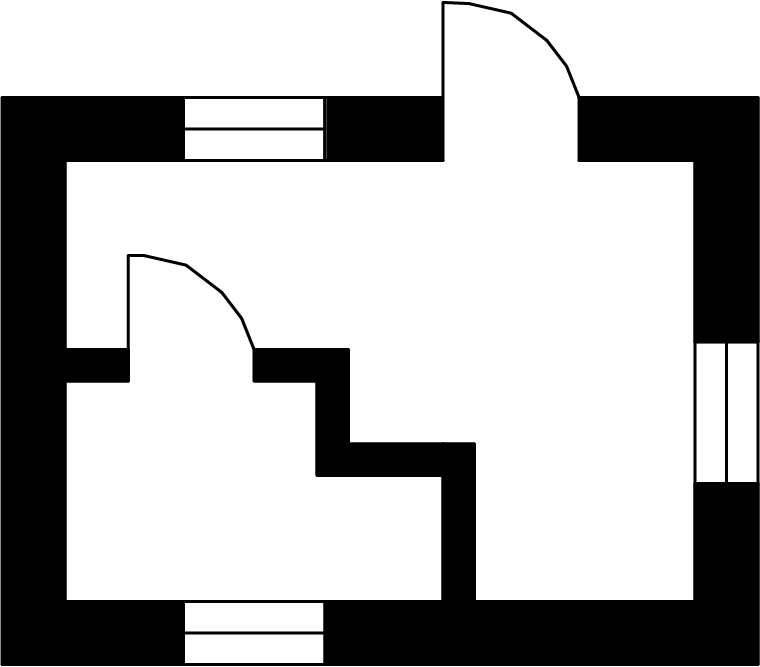
\includegraphics[width=0.5\columnwidth]{fig/scenario2_storey_plan.png}
  \caption{Grundriss des LEGO-Gebäudes.}\label{fig:scenarios:Scenario2 Gebaeudeplan}
\end{figure}

\subsubsection*{Beschreibung}
Zu sehen ist der Plan eines einfachen Hauses mit einem Stockwerk.
Dieses besitzt eine Eingangstür, eine Terrassentür neben einem Fenster und eine Tür, die das Badezimmer vom Hauptraum trennt.
Es gibt breite Außen- und dünne Innenwände.
Dafür müssen zwei Wandtypen definiert werden, die jeweils unterschiedliche Wanddicken vorgeben.
Diese entsprechen in ihren Maßen dem Raster, welches das \textit{LEGO System} vorgibt.
Mehr Informationen darüber werden in Kapitel~\ref{basics:lego} bereitgestellt.
Dickere Wände sollen zwei Noppen breit sein.
Daher wird für diesen Wandtyp ein Grundmodul mit den Maßen 31.8$\times$15.8$\times$9.6 Millimetern und einem Raster von 8$\times$8$\times$9.6 Millimetern gewählt.
Für die dünneren Innenwände soll eine Breite von einer Noppe verwendet werden.
Dies entspricht einem Grundmodul von 15.8$\times$7.8$\times$9.6 Millimetern mit einem gleichbleibenden Raster.
Mögliche Rotationen von Wänden, Fenstern und Türen sind auf 90\textdegree{} Schritte limitiert.
Das stellt im Fall von LEGO eine vertretbare Einschränkung dar, da es ohnehin dem intuitiven Umgang mit dessen Steinen und gleichzeitig dem Baustil der meisten einfachen Gebäuden entspricht.

\subsubsection*{Problemstellungen}
Zusätzlich zu den Teilproblemen des vorhergehenden Szenarios ergeben sich nun weitere Fragestellungen.
Türen und Fenster stellen eine Herausforderung für den Planungsalgorithmus dar, da der Verlauf einer ansonsten durchgängigen Wand dadurch unterbrochen wird und Lücken aufweist.
Diese \glqq{}Lücken\grqq{} werden nachfolgend als Öffnungen bezeichnet.
Öffnungen müssen zunächst im Konstruktionsplaner modelliert werden können, um im Anschluss durch den Planungsalgorithmus weiter verarbeitet zu werden.
Darum muss ein Konzept für Öffnungen erarbeitet werden, um die Definition eines Bereichs innerhalb einer Wand zu ermöglichen, der nicht mit Bausteinen aufgefüllt werden darf.
Wie oben bereits erwähnt, können Wände verschiedene Dicken aufweisen und zusätzlich unter Anwendung unterschiedlicher Grundmodule und Mauerwerksverbände realisiert werden.
Auch diese Eigenschaften müssen sowohl innerhalb des Konstruktionsplaners, als auch im Planungskonzept dieser Arbeit berücksichtigt werden.
Auffällig in diesem Szenario ist auch das Auftreten von T-Kreuzungen zwischen Innen- und Außenwänden.
T- und X-Kreuzungen müssen, ähnlich zu den bereits besprochenen Eckbereichen, zunächst identifiziert und im Anschluss gesondert behandelt werden, da an den Stellen das Einhalten eines bestimmten Mauerwerksverbands besonders komplex ist.
Auch der Übergang zwischen Wänden unterschiedlicher Dicke oder Verband stellt eine weitere Herausforderung dar.
Zusammengefasst ergibt sich durch dieses Szenario folgende neue Liste an Teilproblemen:
\begin{itemize}
  \item Wie werden Öffnungen im Konstruktionsplaner umgesetzt und im Anschluss weiter verarbeitet?
  \item Wie können Wänden Dicke, Grundmodul und Mauerwerksverband zugewiesen werden?
  \item Wie können Übergänge zwischen Wänden verschiedener Dicke oder unterschiedlichem Verband realisiert werden?
  \item Wie können T- und X-Kreuzungen von Eckbereichen unterschieden und dem Mauerwerksverband entsprechend umgesetzt werden? 
\end{itemize}

\subsection{Szenario Fabrikhalle}\label{scenarios:scenario3}
Um das Konzept auch an umfangreicheren Modellen zu testen, wird für dieses Szenario ein Modell einer großen Fabrikhalle erstellt.
In Abbildung~\ref{fig:scenarios:Scenario3 Gebaeudeplan} ist der Grundriss der Fabrikhalle zu sehen.

\subsubsection*{Beschreibung}
Die zu dabei verwendeten Baustein- und Wanddimensionen entsprechen den Größenordnungen, die von dem sogenannten oktametrischen Maßsystem vorgegeben werden.
Informationen dazu sind in Kapitel~\ref{fig:basics:OktametrischeMassordnung} zu finden.
\begin{figure}[ht]
  \centering
  
\includegraphics[width=0.5\columnwidth]{fig/TODO.jpg}
  \caption{Grundriss der Fabrikhalle.}\label{fig:scenarios:Scenario3 Gebaeudeplan}
\end{figure}

\subsubsection*{Problemstellungen}
In diesem Szenario soll vor allem die Laufzeit des erarbeiteten Konzepts auf die Probe gestellt werden.
Dadurch können Teilbereiche davon identifiziert werden, für die eventuell noch Optimierungsbedarf besteht.
%Wie können Eckbereiche zwischen zwei Wänden mit unterschiedlicher Höhe behandelt werden?

\section{Regelbasierte Bauplandeduktion aus einem Bauplanentwurf}\label{scenarios:scenario4}
In dieser Fallstudie wird untersucht wie das Integrieren von Regeln in das erarbeitete Konzept ermöglicht werden kann.
Dabei ist es wünschenswert Regeln erst im Nachgang an den vorangegangenen Schritt des Berechnens eines Bauplanentwurfs zu definieren und auf diesem anzuwenden.
Darum dürfen konkrete Regelbeschreibungen nicht Teil der Programmcodebasis dieser Arbeit sein, sondern müssen auf andere Weise in das Projekt eingefügt werden können.

\subsection*{Problemstellungen}
\begin{itemize}
  \item Wie können Regeln und Regelsets formal definiert werden?
  \item Wie können diese Regelsets zur Auswertung eines Bauplanentwurfs herangezogen werden?
\end{itemize}